\documentclass[a4paper]{article}

\usepackage[utf8]{inputenc}
\usepackage[T1]{fontenc}
\usepackage{mathptmx}
\usepackage{textcomp}
\usepackage{multirow}
\usepackage[UKenglish]{babel}
\usepackage{xcolor}
\definecolor{codegreen}{rgb}{0,0.6,0}
\definecolor{codepurple}{rgb}{0.58,0,0.82}
\usepackage{listings}
\lstdefinestyle{mystyle}{
	commentstyle=\color{codegreen},
	keywordstyle=\color{magenta},
	stringstyle=\color{codepurple},
	showspaces=false,
	showstringspaces=false,
	breaklines=true
}
\lstset{style=mystyle}
\usepackage{amsmath, amssymb}
\usepackage{float}
\usepackage{caption}
\captionsetup{
	aboveskip=4pt,
	belowskip=12pt
}
\DeclareCaptionType{equation}
\usepackage[hidelinks]{hyperref}
\hypersetup{
	colorlinks=false
}
\usepackage[style=ieee]{biblatex}
\bibliography{sources/biblio}

\setlength{\parindent}{0pt}
\setlength{\parskip}{2em}

% figure support
\usepackage{import}
\usepackage{xifthen}
\pdfminorversion=7
\usepackage{pdfpages}
\usepackage{transparent}
\newcommand{\incfig}[1]{%
	\def\svgwidth{\columnwidth}
	\import{./figures/}{#1.pdf_tex}
}

\pdfsuppresswarningpagegroup=1

\begin{document}
\hypersetup{pageanchor=false}
\begin{titlepage}
  \begin{center}

    \textsc{\LARGE Dublin City University}\\[1cm]
    \textsc{\Large Electronic and Computer Engineering}\\[0.5cm]

    {\LARGE \bfseries EE500 Network Performance\\[0.4cm]}
    {\Large \bfseries Assignment 1\\[0.4cm]}

    \begin{figure}[H]
	
\includegraphics{images/Dcu-logo.png}
	\centering
    \end{figure}

    \vskip 2cm
    \emph{Author}\\[0.1cm]
    \noindent\makebox[\textwidth]{%
      \begin{tabular}{ll}%
        Michael Lenehan & michael.lenehan4@mail.dcu.ie \\
	Student Number: & 15410402 \\
    \end{tabular}}\\[0.1cm]

    \vfill

    % Bottom of the page
    % Probably replaced with date of deadline
    {\large{08/12/2019}}

  \end{center}
\end{titlepage}

\hypersetup{pageanchor=true}
\pagenumbering{alph}
\thispagestyle{plain}
\begingroup
\renewcommand{\cleardoublepage}{}
\renewcommand{\clearpage}{}

\LARGE{Declaration}

\endgroup

\vskip 1cm

I declare that this material, which I now submit for assessment, is entirely my
own work and has not been taken from the work of others, save and to the extent
that such work has been cited and acknowledged within the text of my work. I
understand that plagiarism, collusion, and copying are grave and serious
offences in the university and accept the penalties that would be imposed should
I engage in plagiarism, collusion or copying. I have read and understood the
Assignment Regulations set out in the module documentation. I have identified
and included the source of all facts, ideas, opinions, and viewpoints of others
in the assignment references. Direct quotations from books, journal articles,
internet sources, module text, or any other source whatsoever are acknowledged
and the source cited are identified in the assignment references. This
assignment, or any part of it, has not been previously submitted by me or any
other person for assessment on this or any other course of study.

I have read and understood the DCU Academic Integrity and Plagiarism at
\url{https://www4.dcu.ie/sites/default/files/policy/1%20-%20integrity_and_plagiarism\_ovpaa_v3.pdf}
and IEEE referencing guidelines found at
\url{https://loop.dcu.ie/mod/url/view.php?id=448779}.

\vskip 1cm
Signed: \underline{\ \ \ \ \ \ \ \ \ \ \ \ \ \ \ \ \ \ \ \ \ \ \ \ \ \ \ \ \ \ \
\ \ \ \ \ \ } \hspace{20mm}Date: \underline{xx/xx/20xx}

\hspace*{0mm}\phantom{Signed:}Michael Lenehan

\pagebreak

\pagenumbering{arabic}
\tableofcontents
\clearpage
\section{Part 1: Data Transmission over the WiFi Network}
Part 1 of this assignment involves modifying the provided
``wifi-example-sim.cc'' file in order to execute simulations with multiple input
parameters, such as different bitrates, distances between nodes, and number of
nodes.
\subsection{Question A:}
\subsubsection{Part 1:}

\begin{gather*}
test
\end{gather*}
\captionof{equation}{Average Throuhgput (Kbps)}

\begin{gather*}
	test
\end{gather*}
\captionof{equation}{Average Delay (s)}

\begin{gather*}
	test
\end{gather*}
\captionof{equation}{Average Packet Loss Ratio}

\subsubsection{Part 2:}

Within the wifi-example-sim.cc file, the transmission bitrate can be modified in
one of two ways. By modifying the size of the packets being transmit, or by
modifying the delay between packet transmissions. This is shown in the following
calculations:

\begin{gather*}
	R=\frac{rxPackets\times packetSize \times 8}{txTime} \\
	\begin{align*}
		\frac{R\times txTime}{packetSize \times 8} &= rxPackets &
		\undeline{or}& & \frac{R \times txTime}{rxPackets
	\times 8} &= packetSize \\
	\end{align*} \\
	rxPackets=\frac{txTime}{delay}
\end{gather*}
\captionof{equation}{Calculation for Bitrate Modification}

The following table shows the number of packets to be sent (modified by the
delay between packet transmissions), or the size of packet to be sent in order
to meet the required data rates.

\begin{table}[H]
	\centering
	\caption{Bitrate Calculation Results}
	\label{tab:brcalc}
	\begin{tabular}{|c|c|c|c|}
	\hline
	Bitrate & rxPackets & Delay & packetSize \\
	\hline
	1Mbps & 2,500 & $8\times 10^{-3}$ & 625 \\
	1Mbps & 3,750 & $5.3\times 10^{-3}$ & 937.5 \\
	5Mbps & 12,500 & $1.6\times 10^{-3}$ & 3125 \\
	10Mbps & 25,000 & $8\times 10^{-4}$ & 6250 \\
	20Mbps & 50,000 & $4\times 10^{-4}$ & 12,500 \\
	\hline
	\end{tabular}
\end{table}

For the purposes of this section, the delay between the packet transmissions
will be modified. Modifying packet sizes requires using half bytes for packet
sizes.

\begin{gather*}
	test
\end{gather*}
\captionof{equation}{Bitrate of Data Traffic (Kbps)}

\begin{gather*}
test
\end{gather*}
\captionof{equation}{Average Throughput (Kbps}

\begin{gather*}
test
\end{gather*}
\captionof{equation}{Average Delay (s)}

\begin{gather*}
test
\end{gather*}
\captionof{equation}{Average Packet Loss Ratio}

\subsection{Question B:}
This section investigates the effect of distance on throughput, delay and loss
within a single user, single access point system.

\par The throughput, shown below, is constant for the user from distances
between 0 and 110 meters from the access point. Packet loss occurs at
approximately 120 meters, giving greatly decreased throughput. Between 130 and
150 meters, there are no packets received, giving a throughput of 0Kbps.

\begin{gather*}
	Throughput=\frac{rxPackets*1000*8}{txTime} \\
	TP_{0-110}=\frac{400*1000*8}{20}\\
	= 160Kbps\\
	TP_{120}= \frac{13*1000*8}{20}\\
	= 5.2Kbps \\
	TP_{130-150}=\frac{0*1000*8}{20}\\
	= 0Kbps
\end{gather*}
\captionof{equation}{Average Throughput (Kbps) over distances of 0-150m}

The drop of in the throughput is clearly visible within the plot of Figure
\ref{fig:QBthroughput}.

\begin{figure}[H]
	\centering
	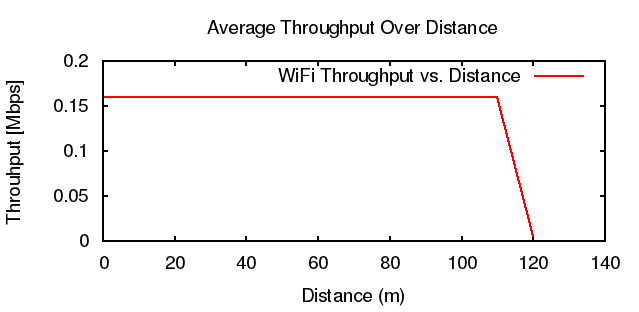
\includegraphics[width=0.8\textwidth]{images/EE500/QB/Images/wifi-throughput}
	\caption{Throughput as measured at distances between 0 and 150 meters}
	\label{fig:QBthroughput}
\end{figure}

The delay, whose values are shown below as read from the database file, begins
to increase at a faster rate between 80 and 110 meters, with much greater
increases between 110 and 120 meters.
\begin{gather*}
	\overline{delay}_0=271582ns \\
	\overline{delay}_{10}=271615ns \\
	\overline{delay}_{20}=271648ns \\
	\overline{delay}_{30}=397353ns \\
	\overline{delay}_{40}=381876ns \\
	\overline{delay}_{50}=490381ns \\
	\overline{delay}_{60}=605123ns \\
	\overline{delay}_{70}=649954ns \\
	\overline{delay}_{80}=835599ns \\
	\overline{delay}_{90}=1279691ns \\
	\overline{delay}_{100}=1574269ns \\
	\overline{delay}_{110}=1723305ns \\
	\overline{delay}_{120}=9362323ns \\
\end{gather*}
\captionof{equation}{Average Delay (ns) over distances of 0-150m}

Beyond a distance of 120m, due to there being a throughput of 0Kbps, there is no
delay value. These values can be seen in Figure \ref{fig:QBdelay}

\begin{figure}[H]
	\centering
	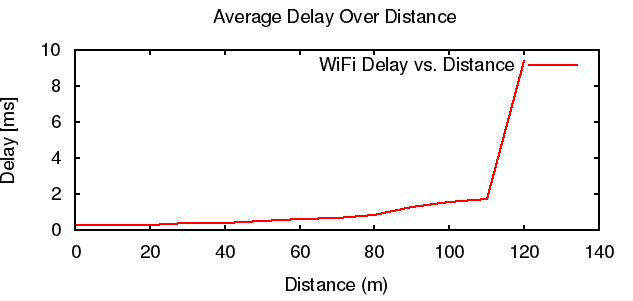
\includegraphics[width=0.8\textwidth]{images/EE500/QB/Images/wifi-delay}
	\caption{Delay as measured at distances between 0 and 150 meters}
	\label{fig:QBdelay}
\end{figure}

For distances between 0 and 110 meters, there is no packet loss due to, as discussed
earlier, all of the packets transmit by the access point are received by the
user.

\par For a distance of 120 meters, the user experiences loss of 96.75\%, and for
distances greater than this, experiences loss of 100\%.

\par The calculations for the packet loss ratio can be seen below:

\begin{gather*}
	PLR=\frac{lostPackets}{rxPackets+lostPackets} \\
	TP_{0-110}=\frac{0}{400+0}\\
	= 0 \\
	TP_{120}= \frac{387}{13+387}\\
	= 0.9675 \\
	TP_{130-150}=\frac{400}{0+400}\\
	= 1
\end{gather*}
\captionof{equation}{Packet Loss Ratio over distances of 0-150m}

\begin{figure}[H]
	\centering
	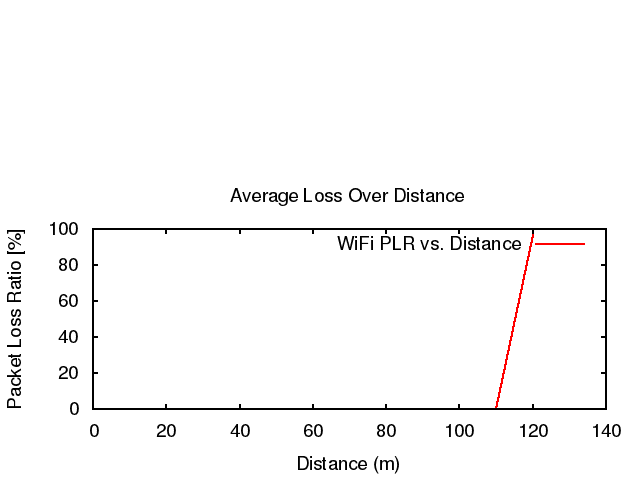
\includegraphics[width=0.8\textwidth]{images/EE500/QB/Images/wifi-loss}
	\caption{Packet Loss Ratio as measured at distances between 0 and 150
	meters}
	\label{fig:QBloss}
\end{figure}

\subsection{Question C:}
\subsubsection{Part 1:}

\begin{gather*}
test
\end{gather*}
\captionof{equation}{Average Throuhgput (Kbps)}

\begin{gather*}
	test
\end{gather*}
\captionof{equation}{Average Delay (s)}

\begin{gather*}
	test
\end{gather*}
\captionof{equation}{Average Packet Loss Ratio}

\subsubsection{Part 2:}

Within the wifi-example-sim.cc file, the transmission bitrate can be modified in
one of two ways. By modifying the size of the packets being transmit, or by
modifying the delay between packet transmissions. This is shown in the following
calculations:

\begin{gather*}
	R=\frac{rxPackets\times packetSize \times 8}{txTime} \\
	\begin{align*}
		\frac{R\times txTime}{packetSize \times 8} &= rxPackets &
		\undeline{or}& & \frac{R \times txTime}{rxPackets
	\times 8} &= packetSize \\
	\end{align*} \\
	rxPackets=\frac{txTime}{delay}
\end{gather*}
\captionof{equation}{Calculation for Bitrate Modification}

The following table shows the number of packets to be sent (modified by the
delay between packet transmissions), or the size of packet to be sent in order
to meet the required data rates.

\begin{table}[H]
	\centering
	\caption{Bitrate Calculation Results}
	\label{tab:brcalc}
	\begin{tabular}{|c|c|c|c|}
	\hline
	Bitrate & rxPackets & Delay & packetSize \\
	\hline
	1Mbps & 2,500 & $8\times 10^{-3}$ & 625 \\
	1Mbps & 3,750 & $5.3\times 10^{-3}$ & 937.5 \\
	5Mbps & 12,500 & $1.6\times 10^{-3}$ & 3125 \\
	10Mbps & 25,000 & $8\times 10^{-4}$ & 6250 \\
	20Mbps & 50,000 & $4\times 10^{-4}$ & 12,500 \\
	\hline
	\end{tabular}
\end{table}

For the purposes of this section, the delay between the packet transmissions
will be modified. Modifying packet sizes requires using half bytes for packet
sizes.

\begin{gather*}
	test
\end{gather*}
\captionof{equation}{Bitrate of Data Traffic (Kbps)}

\begin{gather*}
test
\end{gather*}
\captionof{equation}{Average Throughput (Kbps}

\begin{gather*}
test
\end{gather*}
\captionof{equation}{Average Delay (s)}

\begin{gather*}
test
\end{gather*}
\captionof{equation}{Average Packet Loss Ratio}

\subsubsection{Part 3:}

\begin{figure}[H]
	\centering
	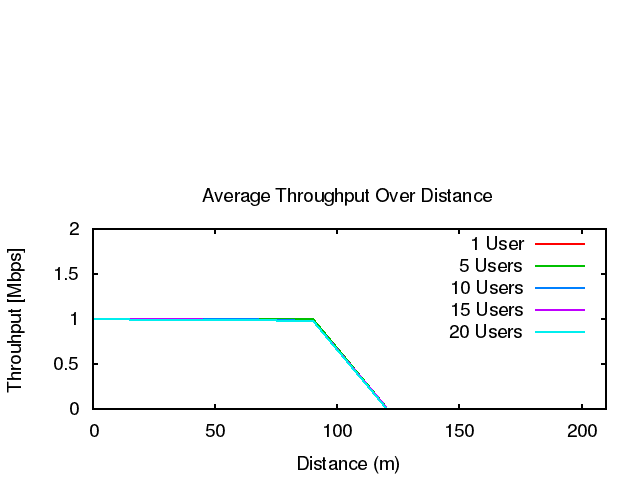
\includegraphics[width=0.8\textwidth]{images/EE500/QC/P3/Images/wifi-throughput}
	\caption{Throughput for systems with 0 to 20 users, over distances from
	0 to 150 meters}
	\label{fig:QCP3throughput}
\end{figure}

\begin{table}[H]
	\centering
	\caption{Throughput Values (Kbps) for 1-20 User Systems at Distances of 0-150m}
	\label{tab:QCP3TPTable}
	\begin{tabular}{|c|c|c|c|c|c|}
		\hline
		Distance & 1 User & 5 Users & 10 Users & 15 Users & 20 Users\\
		\hline
		0 & 1000 & 1000 & 1000 & 1000 & 1000\\
		30 & 1000 & 1000 & 1000 & 1000 & 990.8\\
		60 & 1000 & 1000 & 1000 & 986 & 986\\
		90 & 1000 & 1000 & 974.8 & 975.6 & 975.6\\
		120 & 17.6 & 18.4 & 18.4 & 17.6 & 15.2\\
		\hline
	\end{tabular}
\end{table}

\begin{figure}[H]
	\centering
	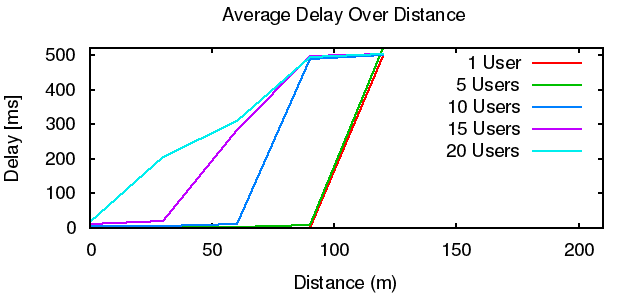
\includegraphics[width=0.8\textwidth]{images/EE500/QC/P3/Images/wifi-delay}
	\caption{Delay for systems with 0 to 20 users, over distances from 0 to
	150 meters}
	\label{fig:QCP3delay}
\end{figure}

\begin{table}[H]
	\centering
	\caption{Delay Values (ms) for 1-20 User Systems at Distances of 0-150m}
	\label{tab:QCP3TPTable}
	\begin{tabular}{|c|c|c|c|c|c|}
		\hline
		Distance & 1 User & 5 Users & 10 Users & 15 Users & 20 Users\\
		\hline
		0 & 0.194653 & 1.57338 & 5.6031 & 11.2192 & 18.5429\\
		30 & 0.347009 & 2.32888 & 7.16022 & 19.1675 & 203.886\\
		60 & 0.566218 & 3.44795 & 12.5859 & 283.532 & 310.421\\
		90 & 1.27689 & 8.00458 & 488.852 & 496.113 & 494.484\\
		120 & 497.965 & 523.288 & 499.474 & 504.065 & 504.108\\
		\hline
	\end{tabular}
\end{table}

\begin{figure}[H]
	\centering
	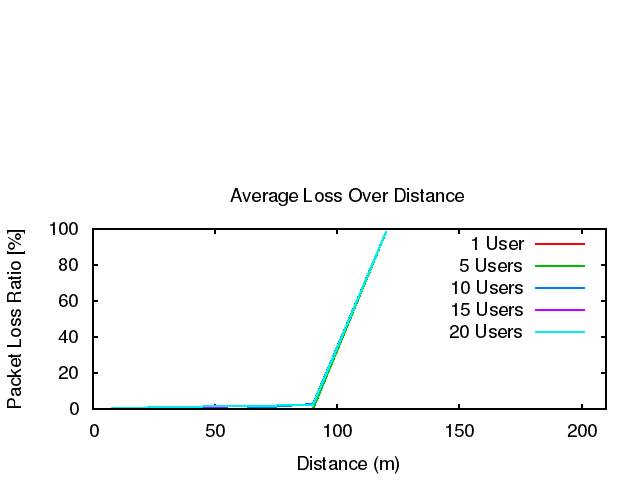
\includegraphics[width=0.8\textwidth]{images/EE500/QC/P3/Images/wifi-loss}
	\caption{Loss for systems with 0 to 20 users, over distances from 0 to
	150 meters}
	\label{fig:QCP3loss}
\end{figure}

\begin{table}[H]
	\centering
	\caption{Packet Loss Ratio for 1-20 User Systems at Distances of 0-150m}
	\label{tab:QCP3TPTable}
	\begin{tabular}{|c|c|c|c|c|c|}
		\hline
		Distance & 1 User & 5 Users & 10 Users & 15 Users & 20 Users\\
		\hline
		0 & 0 & 0 & 0 & 0 & 0\\
		30 & 0 & 0 & 0 & 0 & 0.92\\
		60 & 0 & 0 & 0 & 1.4 & 1.4\\
		90 & 0 & 0 & 2.52 & 2.44 & 2.44\\
		120 & 98.24 & 98.16 & 98.16 & 98.24 & 98.48\\
		\hline
	\end{tabular}
\end{table}

\section{Part 2: Results and Comparison and Analysis}
\subsubsection{Part 2:}

Within the wifi-example-sim.cc file, the transmission bitrate can be modified in
one of two ways. By modifying the size of the packets being transmit, or by
modifying the delay between packet transmissions. This is shown in the following
calculations:

\begin{gather*}
	R=\frac{rxPackets\times packetSize \times 8}{txTime} \\
	\begin{align*}
		\frac{R\times txTime}{packetSize \times 8} &= rxPackets &
		\undeline{or}& & \frac{R \times txTime}{rxPackets
	\times 8} &= packetSize \\
	\end{align*} \\
	rxPackets=\frac{txTime}{delay}
\end{gather*}
\captionof{equation}{Calculation for Bitrate Modification}

The following table shows the number of packets to be sent (modified by the
delay between packet transmissions), or the size of packet to be sent in order
to meet the required data rates.

\begin{table}[H]
	\centering
	\caption{Bitrate Calculation Results}
	\label{tab:brcalc}
	\begin{tabular}{|c|c|c|c|}
	\hline
	Bitrate & rxPackets & Delay & packetSize \\
	\hline
	1Mbps & 2,500 & $8\times 10^{-3}$ & 625 \\
	1Mbps & 3,750 & $5.3\times 10^{-3}$ & 937.5 \\
	5Mbps & 12,500 & $1.6\times 10^{-3}$ & 3125 \\
	10Mbps & 25,000 & $8\times 10^{-4}$ & 6250 \\
	20Mbps & 50,000 & $4\times 10^{-4}$ & 12,500 \\
	\hline
	\end{tabular}
\end{table}

For the purposes of this section, the delay between the packet transmissions
will be modified. Modifying packet sizes requires using half bytes for packet
sizes.

\begin{gather*}
	test
\end{gather*}
\captionof{equation}{Bitrate of Data Traffic (Kbps)}

\begin{gather*}
test
\end{gather*}
\captionof{equation}{Average Throughput (Kbps}

\begin{gather*}
test
\end{gather*}
\captionof{equation}{Average Delay (s)}

\begin{gather*}
test
\end{gather*}
\captionof{equation}{Average Packet Loss Ratio}

\clearpage
\section{Appendix}
\subsection{Bash Scripts}
The following bash scripts were used to execute the simulations in ns-3, to save
the outputs to .db files, and to plot the outputs from the simulation.
\subsubsection{Question A Part 1 Bash Script}
\lstinputlisting[language=bash]{sections/Appendix/EE500/wifi-p1qap1.sh}
\subsubsection{Question A Part 2 Bash Script}
\lstinputlisting[language=bash]{sections/Appendix/EE500/wifi-p1qap2.sh}
\subsubsection{Question B Bash Script}
\lstinputlisting[language=bash]{sections/Appendix/EE500/wifi-p1qb.sh}
\subsubsection{Question C Part 1 Bash Script}
\lstinputlisting[language=bash]{sections/Appendix/EE500/wifi-p1qcp1.sh}
\subsubsection{Question C Part 2 Bash Script}
\lstinputlisting[language=bash]{sections/Appendix/EE500/wifi-p1qcp2.sh}
\subsubsection{Question C Part 3 Bash Script}
\lstinputlisting[language=bash]{sections/Appendix/EE500/wifi-p1qcp3.sh}

\subsection{C++ Files}
The following script is a modified version of the provided code required to
execute the simulation within ns-3.
\subsubsection{C++ Simulation File}
\lstinputlisting[language=C++]{sections/Appendix/EE500/wifi-example-sim.cc}

\subsection{Gnuplot Files}
The following scripts are used to plot the values extracted from the .db files
output from the simulations.
\subsubsection{Question A Part 1 Bash Script}
\lstinputlisting[language=Gnuplot]{sections/Appendix/EE500/wifi-p1qap1.gnuplot}
\subsubsection{Question A Part 2 Bash Script}
\lstinputlisting[language=Gnuplot]{sections/Appendix/EE500/wifi-p1qap2.gnuplot}
\subsubsection{Question B Bash Script}
\lstinputlisting[language=Gnuplot]{sections/Appendix/EE500/wifi-p1qb.gnuplot}
\subsubsection{Question C Part 1 Bash Script}
\lstinputlisting[language=Gnuplot]{sections/Appendix/EE500/wifi-p1qcp1.gnuplot}
\subsubsection{Question C Part 2 Bash Script}
\lstinputlisting[language=Gnuplot]{sections/Appendix/EE500/wifi-p1qcp2.gnuplot}
\subsubsection{Question C Part 3 Bash Script}
\lstinputlisting[language=Gnuplot]{sections/Appendix/EE500/wifi-p1qcp3.gnuplot}

\clearpage
\printbibliography
\end{document}
